 \documentclass[c]{beamer}
%\documentclass{beamer}
\listfiles

\mode<presentation>
{
  %\usetheme[deutsch,titlepage0]{KIT}
\usetheme[deutsch]{KIT}
% \usetheme{KIT}

%%  \usefonttheme{structurebold}

  \setbeamercovered{transparent}

  \setbeamertemplate{enumerate items}[circle]
  %\setbeamertemplate{enumerate items}[ball]

}
\usepackage{babel}
\date{}
%\DateText

\newlength{\Ku}
\setlength{\Ku}{1.43375pt}

\usepackage[utf8]{inputenc}
\usepackage[TS1,T1]{fontenc}
\usepackage{array}
\usepackage{multicol}
\usepackage{lipsum}
\usepackage[]{algorithm2e}
\usepackage{amsmath}
\usepackage{color}

\usenavigationsymbols
%\usenavigationsymbols[sfHhdb]
%\usenavigationsymbols[sfhHb]

\subtitle{Algorithmen I SS 14}
\author[]{Lena Winter}

\AuthorTitleSep{\relax}

\institute[ITI]{Institut für Theoretische Informatik}

\TitleImage[width=\titleimagewd]{images/title}

\newlength{\tmplen}

\newcommand{\verysmall}{\fontsize{6pt}{8.6pt}\selectfont}

\title[Algorithmen I SS 14]{Tutorium 6}

\usepackage{alltt}

\TitleImage[width=\titleimagewd]{images/title}

\definecolor{english}{rgb}{0.0, 0.5, 0.0}

\begin{document}

\begin{frame}
  \maketitle
\end{frame}

\begin{frame}
	\begin{center}
		\Huge
		Heaps
	\end{center}
\end{frame}

\begin{frame}{Heaps}
	(Binärer) Baum mit zusätzlicher Eigenschaft:
	\begin{itemize}
		\item Eltern sind kleiner gleich ihren Kindern: $\forall v: parent(v) \leq v$
		\item Auch umgekehrt möglich (Max-Heap)
	\end{itemize}

\end{frame}

\begin{frame}{Heapoperationen}
	\begin{itemize}
		\item Minimum finden in $\mathcal{O}(1)$ (Wurzel betrachten)
		\item Einfügen in $\mathcal{O}(\log{n})$
		\item Wurzel extrahieren in $\mathcal{O}(\log{n})$
		\item Heap aufbauen in $\mathcal{O}(n)$
	\end{itemize}

\end{frame}

\begin{frame}{Implementierung}
	Im Computer effizient als Array darstellbar: \\
	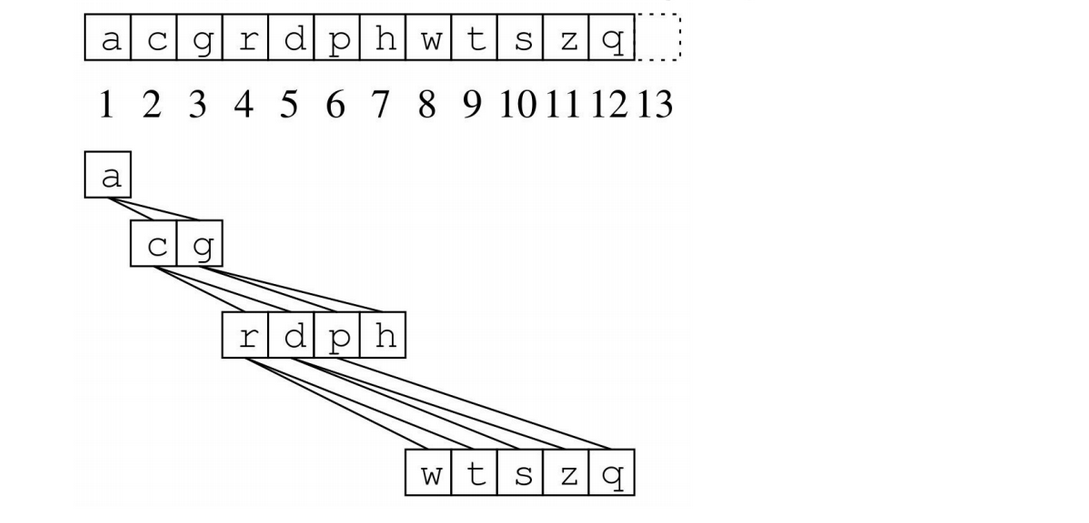
\includegraphics[scale=0.2]{images/heapArray.png} \\
\end{frame}

\begin{frame}{Baumnavigation in Arraydarstellung}
	\begin{description}
		\item[leftChild(i):] heap[$2 i$]
		\item[rightChild(i):] heap[$2 i + 1$]
		\item[parent(i):] heap[$\lfloor \frac{i}{2} \rfloor$]
	\end{description}
	\begin{itemize}
		\item Ein Heap der Höhe h hat mindestens $2^{h - 1} $ und maximal $ 2^{h} - 1$ Elemente
		\item Ein Heap mit n Elementen hat die Höhe $1 + \lfloor \log_2(n) \rfloor$
	\end{itemize}
\end{frame}

\begin{frame}{Heapoperationen: insert}
	\begin{enumerate}
		\item Einfügen des neuen Elements an letzter Stelle
		\item Heap-Eigenschaft ist jetzt möglicherweise dort verletzt
		\item Schiebe Element so lange nach \emph{oben}, bis Heap-Eigenschaft wiederhergestellt ist (siftUp)
		\item Also: Vergleiche jeweils mit dem Elternelement und vertausche, falls es größer ist
	\end{enumerate}
\end{frame}

\begin{frame}{Heapoperationen: deleteMin}
	\begin{enumerate}
		\item Lösche erstes Element und ersetze es durch letztes Element
		\item Heap-Eigenschaft nun möglicherweise dort verletzt
		\item Schiebe Element so lange nach \emph{unten}, bis Heap-Eigenschaft wiederhergestellt ist (siftDown)
		\item Also: Vergleiche jeweils mit Kindelementen und vertausche mit dem kleineren
	\end{enumerate}
\end{frame}

\begin{frame}{Heapoperationen: buildHeap}
	\begin{enumerate}
		\item Füge Elemente ohne Beachtung der Heap-Eigenschaft ein
		\item Stelle Heap-Eigenschaft ebenenweise von unten wieder her
		\item Führe siftDown auf alle Elemente, beginnend bei der vorletzten Ebene aus
	\end{enumerate}
\end{frame}

\begin{frame}{Heapsort}
	\begin{itemize}
		\item Benutze \emph{buildHeap()} um Heap aufzubauen
		\item $n$ mal \emph{deleteMin()} um Minimum zu extrahieren
		\item insgesamt also Laufzeit $\mathcal{O}(n \log{n})$
		\item echt in-place
	\end{itemize}
\end{frame}

\begin{frame}{Aufgabe: Heapsort}
	Sortiere die Folge $\langle 65, 32, 85, 37, 84, 64, 3, 31, 47 \rangle$ mit Heapsort aufsteigend.
\end{frame}

\begin{frame}{Kreativaufgabe: Pancake-Sorting}
	\begin{itemize}
		\item \textbf{gegeben:} Stapel von \emph{n} Pancakes, Pancake-Flipper mit dem man die obersten \emph{k} Pancakes drehen kann ($ k \leq n $).
		\item \textbf{gesucht:} Schnelles Verfahren zum Sortieren der Pancakes.
	\end{itemize}
\end{frame}

\begin{frame}{Lösung: Pancake-Sorting}
	\begin{itemize}
		\item Größten Pancake nach oben flippen und dann Stapel komplett wenden. Anschließend genauso für die kleineren Panecakes.  $ \Rightarrow $ Laufzeit: $2n$
		\item Man kann allerdings nach dem Zweitkleinsten aufhören. $ \Rightarrow $ Laufzeit: $2(n - 1)$
		\item Hat man den drittgrößten Pancake erreicht, gibt es für die kleinsten nur 2 Möglichkeiten, d.h. muss man maximal einmal drehen. $ \Rightarrow $ Laufzeit: $2(n-1) - 1 = 2n - 3$
	\end{itemize}

\end{frame}

\begin{frame}{Kreativaufgabe: Spaghetti-Sort}
	\begin{itemize}
		\item \textbf{gegeben:} Liste mit \emph{n} Elementen $\in \mathbb{N}$, eine Packung Spaghetti mit mindestens \emph{n} Spaghetti.
		\item \textbf{gesucht:} Algorithmus zum Sortieren der Liste mit Hilfe der Spaghetti in $\mathcal{O}(n)$.
	\end{itemize}
\end{frame}

\begin{frame}
	\frametitle{Tree}
	\begin{center}
		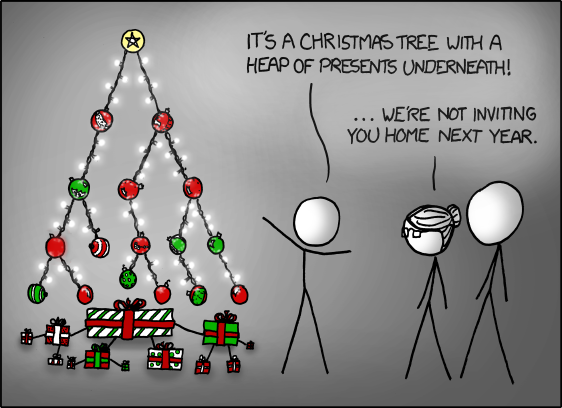
\includegraphics[width=\textwidth,height=\textheight,keepaspectratio]{images/tree}
	\end{center}
\end{frame}

\end{document}
